\documentclass{llncs}

\usepackage{epsfig}
\usepackage{graphicx}
\usepackage{color}
\usepackage{amsfonts}
\usepackage{amsmath}
\usepackage{mathabx}
%\usepackage{hyperref}
%\usepackage{subfigure}
%\usepackage[colorinlistoftodos, textwidth=3.2cm, shadow]{todonotes}

\usepackage{algorithm}
\usepackage{fixltx2e}
\usepackage{algpseudocode}

\usepackage{multirow}

% To use Call inside another Call (algorithms)
\MakeRobust{\Call}


%%%%%%%%%%%%%%%%%%%%%%%%%%%%%%%%%%%%%%%%%%
%
% Title
%
%%%%%%%%%%%%%%%%%%%%%%%%%%%%%%%%%%%%%%%%%%
\title{RTS AI Problems and Techniques
%\thanks{Supported by ...}
}

\author{Santiago~Onta\~{n}\'{o}n\inst{1} \and 
		Gabriel~Synnaeve\inst{2} \and
		Alberto~Uriarte\inst{1} \and
		Florian~Richoux\inst{3} \and
		David~Churchill\inst{4} \and
		Mike~Preuss\inst{5}
		}

\institute{
	Computer Science Department at Drexel University, Philadelphia, PA, USA. \\
	\email{\{santi,albertouri\}@cs.drexel.edu}
\and
	Cognitive Science and Psycholinguistics (LSCP) of ENS Ulm, Paris, France. \\
	\email{gabriel.synnaeve@gmail.com}
\and
	Nantes Atlantic Computer Science Laboratory (LINA), Univ. Nantes, France.\\
	\email{florian.richoux@univ-nantes.fr}
\and
	Computing Science Department of the University of Alberta, Edmonton, Canada. \\
	\email{cdavid@cs.ualberta.ca}
\and
	Department of Computer Science of Technische Universit{\"a}t Dortmund, Germany.
	\email{mike.preuss@cs.tu-dortmund.de}
}

\begin{document}

\maketitle

\begin{abstract}
  This is the abstract.
\end{abstract}


\section{Introduction}\label{sec:intro}
The  field of  Real-Time Strategy  (RTS) game  Artificial Intelligence
(AI) has advanced significantly since Michael Buro's call for research
in this area \cite{Buro03rts}. Specially, competitions like the ``ORTS
RTS  Game AI  Competition''  (held  from 2006  to  2009), the  ``AIIDE
StarCraft AI Competition'' (held since  2010), and the ``CIG StarCraft
RTS AI Competition'' (held since  2011) have motivated the exploration
of many  AI approaches  in the  context of  RTS AI.  We will  list and
classify these approaches, explain  their strengths and weaknesses and
conclude on what is left to achieve human-level RTS AI.

Complex  dynamic  environments,  where neither  perfect  nor  complete
information  about the  current state  or  about the  dynamics of  the
environment are available, pose  significant challenges for artificial
intelligence. Road traffic, finance, or weather forecasts are examples
of such large, complex, real-life  dynamic environments. RTS games can
be seen  as a simplification  of one such real-life  environment, with
simpler dynamics in a finite and smaller world, although still complex
enough to  study some  of the key  interesting problems  like decision
making under  uncertainty or  real-time adversarial  planning. Finding
efficient techniques for tackling these problems on RTS games can thus
benefit other  AI disciplines and  application domains, and  also have
concrete and direct applications in the ever growing industry of video
games.

% Some other arguments for the motivation: 
% 1. It's fun 
% 2. Togelius' argument: Some problems  are very similar than the ones
% in  robotics (decision  making, pathfinding,  ...).  However  RTS AI
% does  not have  the same  limitations for  running experiments:  few
% hardware constraints (we just need  a computer), we can have control
% on the time flow, we can run many experiments in parallel, ...


This article aims to  provide an overview on what is  the state of the
art  in  RTS AI,  with  a  particular emphasis  on  the  work done  in
StarCraft.  It is organized as follows: 
{\color{blue} TODO}

% Section~\ref{sec:rts}
% introduces RTS games, in particular the game StarCraft, and their main
% AI challenges.  Section~\ref{sec:review} reviews  the existing work on
% tackling  these   challenges  in  RTS   games.   Section~\ref{sec:bot}
% analyzes  several current  state of  the art  RTS game  playing agents
% (called  {\em  bots}),  selected   from  the  participants  to  annual
% StarCraft  AI  competitions.   Section~\ref{sec:competition}  presents
% results of  the recent annual competitions  held at the AIIDE  and CIG
% conferences  and  a  StarCraft bot  game  ladder\footnote{An  extended
%   tournament,   which   can    potentially   go   on   indefinitely.}.
% Section~\ref{sec:questions}  compiles  open   questions  in  RTS  game
% AI. Finally, the paper concludes on discussions and perspectives.


\section{Real-Time Strategy Games}\label{sec:rts}

Real-Time Strategy is a sub-genre of strategy games where players need
to  build an  economy (gathering  resources and  building a  base) and
military power (training units  and researching technologies) in order
to defeat  their opponents  (destroying their army  and base).  From a
theoretical point of view, the  main differences between RTS games and
traditional board games such as Chess or Go are:

\begin{itemize}
\item  They are  {\em simultaneous  move} games,  where more  than one
  player  can issue  actions  at the  same  time. Additionally,  these
  actions are {\em durative}, i.e.  actions are not instantaneous, but
  take some amount of time to complete.
\item RTS games  are ``real-time'', which actually means  is that each
  player  has  a  very  small  amount  of  time  to  decide  the  next
  move. Compared to  Chess, where players may have  several minutes to
  decide the next action, in StarCraft, the game executes at 24 frames
  per second, which means that players  can act as fast as every 42ms,
  before the game state changes.
\item Most  RTS games are  partially observable: players can  only see
  the part of the  map that has been explored. This  is referred to as
  the {\em fog-of-war}.
\item Most RTS games are non-deterministic. Some actions have a chance
  of success.
\item And  finally, the complexity  of these  games, both in  terms of
  state space size and in terms of number of actions available at each
  decision cycle is very large. For  example, the state space of Chess
  is typically  estimated to  be around  $10^{50}$, heads  up no-limit
  Texas holdem  poker around $10^{80}$,  and Go around  $10^{170}$. In
  comparison,  the  state space  of  StarCraft  in  a typical  map  is
  estimated to be  many orders of magnitude larger than  any of those,
  as discussed in the next section.
\end{itemize}

For those reasons, standard techniques  used for playing classic board
games, such as  game tree search, cannot be directly  applied to solve
RTS games without the definition of some level of abstraction, or some
other simplification. Interestingly enough, humans  seem to be able to
deal with the  complexity of RTS games, and are  still vastly superior
to       computers      in       these       types      of       games
\cite{burochurchill2012aimagazine}.   For  those   reasons,  a   large
spectrum of techniques  have been attempted to deal  with this domain,
as we will describe below. The remainder of this section is devoted to
describe StarCraft  as a research  testbed, and on detailing  the open
challenges in RTS game AI.

\subsection{StarCraft}\label{subsec:StarCraft}

{\em StarCraft: Brood  War} is an immensely popular  RTS game released
in   1998  by   Blizzard  Entertainment.   StarCraft  is   set  in   a
science-fiction based universe where the player must choose one of the
three  races: Terran,  Protoss or  Zerg.  One of  the most  remarkable
aspects  of StarCraft  is  that  the three  races  are extremely  well
balanced:

\begin{itemize}
\item Terrans provide  units that are versatile and  flexible giving a
  balanced option between Protoss and Zergs.
\item  Protoss   units  have   lengthy  and   expensive  manufacturing
  processes, but they are strong and resistant.  These conditions make
  players follow a strategy of quality over quantity.
\item Zergs, the insectoid race, units are cheap and weak. They can be
  produced fast, encouraging players to overwhelm their opponents with
  sheer numbers.
\end{itemize}

% What about copyright problems with this screenshot?
% Figure~\ref{fig:StarCraft} shows  a screenshot of StarCraft  showing a
% player playing the Terran race. 
In order to win a StarCraft  game, players must first gather resources
(minerals  and Vespene  gas). As  resources become  available, players
need to allocate them for creating more buildings (which reinforce the
economy, and allow players to  create units or unlock stronger units),
research  new technologies  (in order  to  use new  unit abilities  or
improve the units)  and train attack units. Units  must be distributed
to  accomplish different  tasks  such as  reconnaissance, defense  and
attack.  While  performing all  of those tasks,  players also  need to
strategically understand the geometry of the  map at hand, in order to
decide where to place new buildings  (concentrate in a single area, or
expand  to  different  areas)  or where  to  set  defensive  outposts.
Finally, when  offensive units of  two players meet, each  player must
quickly maneuver each  of the units in order to  fight a battle, which
requires quick and reactive control of each of the units.

% \begin{figure}
%     \centering
%     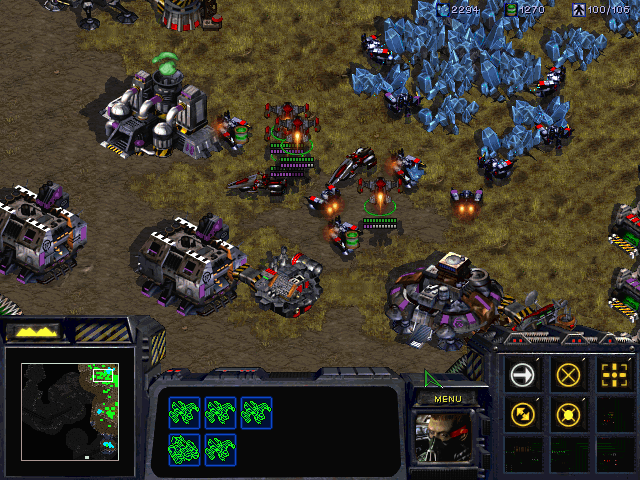
\includegraphics[width=0.8\columnwidth]{figures/starcraft1.png}
%     \caption{A screenshot of \emph{StarCraft: Brood War}.}
%     \label{fig:StarCraft}
% \end{figure}

A typical  StarCraft map is defined  as a rectangular grid,  where the
$width \times  height$ of  the map  is measured in  the number  of $32
\times 32$ squares of pixels, also  known as build tiles. However, the
resolution of  walkable areas is  in squares  of $8 \times  8$ pixels,
also known as  walk tiles. The typical dimensions for  maps range from
$64  \times 64$  to  $256 \times  256$ build  tiles.  Each player  can
control  up to  200 units  (plus  an unlimited  number of  buildings).
Moreover,  each different  race contains  between 30  to 35  different
types of units  and buildings, most of them with  a significant number
of  special abilities.  All these  factors together  make StarCraft  a
significant  challenge, in  which humans  are still  much better  than
computers.      For     instance,      in     the      game     ladder
iCCup\footnote{http://www.iccup.com/StarCraft/} where users are ranked
by their current point totals ($E$ being the lowest possible rank, and
$A^+$  and  $Olympic$ being  the  second  highest and  highest  ranks,
respectively), the best  StarCraft AI bots are ranked  between $D$ and
$D^+$,  where average  amateur players  are ranked  between $C^+$  and
$B$. For comparison, StarCraft professional players are usually ranked
between $A^-$ and $A^+$.

From a theoretical point of view,  the state space of a StarCraft game
for a given map is enormous.  For example, consider a $128 \times 128$
map. At any given moment there might be between 50 to 400 units in the
map,  each of  which might  have a  complex internal  state (remaining
energy  and hit-points,  action  being executed,  etc.). This  quickly
leads to an immense number of  possible states (way beyond the size of
smaller games, such as Chess or Go). For example, just considering the
location of  each unit (with  $128 \times 128$ possible  positions per
unit),  and 400  units, gives  us  an initial  number of  $16384^{400}
\approx 10^{1685}$. If we add the  other factors playing a role in the
game, we obtain even larger numbers.

Another way to measure the complexity of the game is by looking at the
branching factor,  $b$, and the  depth of  the game, $d$,  as proposed
in~\cite{Gaby}, with  a total game  complexity of $b^d$. In  Chess, $b
\approx 35$  and $d \approx  80$. In more  complex games, like  Go, $b
\approx  30$ to  $300$, and  $d  \approx 150$  to $200$.  In order  to
determine the  branching factor in StarCraft  when an AI plays  it, we
must have in mind, that the  AI can issue actions simultaneously to as
many  units in  the  game as  desired. Thus,  considering  that, in  a
typical game, a player controls between 50 to 200 units, the branching
factor  would be  between $u^{50}$  and  $u^{200}$, where  $u$ is  the
average number of actions each unit can execute.  Estimating the value
of $u$ is not easy, since the  number of actions a unit can execute is
highly  dependent   on  the  context.   Let  us  make   the  following
assumptions: 1) at most 16 enemy units  will be in range of a friendly
unit (larger values  are possible, but unlikely), 2) when  an AI plays
StarCraft, it only makes sense to  consider movement in the 8 cardinal
directions per unit  (instead of assuming that the player  can issue a
``move'' command to anywhere in the map  at any point in time), 3) for
``build'' actions,  we consider that  SCVs (Terran worker  units) only
build in their  current location (otherwise, if they need  to move, we
consider  that  as  first  issuing  a  ``move''  action,  and  then  a
``build''), and  4) let's  consider only the  {\em Terran}  race. With
those assumptions,  units in  StarCraft can  execute between  1 (units
like ``Supply  Depots'', whose only  action is  to be ``idle'')  to 43
actions (Terran ``Ghosts''), with typical values around 20 to 30. Now,
if we have in mind that actions have cool-down times, and thus not all
units can  execute all of  the actions at every  frame, we can  take a
conservative estimation  of about $10$  possible actions per  unit per
game frame. This results in  a conservative estimate for the branching
factor  between $b  \in  [10^{50},10^{200}]$,  only considering  units
(ignoring the actions buildings can execute).
% Assuming  a conservative  value for  $u$  of about  $30$ (moving  to
% nearby positions, attacking units in range, using special abilities,
% etc.), we  obtain a  branching factor of  $b$ between  $30^{50}$ and
% $30^{200}$.
Now, to  compute $d$, we simply  consider the fact that  typical games
last for  about 25  minutes, which  results in  $d \approx  36000$ (25
minutes $\times$ 60 seconds $\times$ 24 frames per second).


% In StarCraft,  humans can issue only  one action at a  time (this is
% because of  the GUI  used by  the game,  computer players  can issue
% several  actions, to  different  units, at  any  given time),  thus,
% assuming a  player controls between 50  to 200 units, and  that each
% unit can execute  between 4 to 20  actions (moving in each  of the 4
% cardinal  directions,   attacking  units   in  range,   use  special
% abilities, etc.), we estimate the branching factor for human players
% to be around $b \approx 200  - 4000$. Good players can execute about
% 300 actions per minute, and the typical length of a game is about 25
% minutes. Thus, $d \approx 7500$.

% However, this  is a weak indication  of the complexity of  the game,
% since many  of those states  would never be  reached in a  game. For
% that  reason, it  is  more useful  to  just think  in  terms of  the
% branching factor  and depth  of a  game, when a  human plays  it. In
% Chess,  the branching  factor is  around  35 and  the depth,  around
% 80. In Go, the  branching factor is between 30 to  300 and the depth
% 150 to 200. In StarCraft, humans can execute about ...


% From Gabriel's dissertation:
% ------------------------------------
%How does the state of possible actions grow? To measure this, we
%used a measure from perfect information zero-sum games (as Checkers,
%Chess and Go): the branching factor* b and the depth d of a typical
%game. The complexity of a game (for taking a decision) is proportional
%to bd.
%[...]
%In RTS games, b = 200 is a lower bound (in StarCraft we may have
%between 50 to 400 units to control), and very good amateurs and
%professional players perform more than 300 actions per minute. As
%StarCraft is a simultaneous move, multi-units game, a strict number
%for b would be |actions||units| (actions account for atomic moves and
%abilities), thus for StarCraft b would be around 30^{60}. Strictly
%speaking, for a StarCraft game, d = 24  game_seconds (24 game frames
%per second), with a game duration of 25 minutes, this gives d =
%36,000, thus b^d Å 30^{60^{36000}} .


\subsection{Challenges in RTS Game AI}\label{subsec:challenges}

Early research  in AI  for RTS  games \cite{Buro03rts}  identified the
following six challenges:
\begin{itemize}
\item Resource management
\item Decision making under uncertainty
\item Spatial and temporal reasoning
\item Collaboration (between multiple AIs)
\item Opponent modeling and learning
\item Adversarial real-time planning
\end{itemize}

While there  has been  a significant  work in  many, others  have been
untouched (e.g. collaboration). Moreover, recent research in this area
has identified several additional research  challenges, such as how to
exploit the massive amounts  of existing domain knowledge (strategies,
build-orders,  replays,  and  so   on).  Below,  we  describe  current
challenges in RTS Game AI, grouped in six main different areas.

%\begin{itemize}
%\item Task Decomposition (or ``Architecture'')
%\item Integration of Domain Knowledge
%\item Reasoning with Uncertainty (including information gathering)
%\item Opponent Modeling  and Adaptation: opponent modeling  is key if
%  we  have  to  adapt  our  strategy.  As  different  strategies  are
%  dominating each  others, forming  multiple Nash equilibria,  the AI
%  has to be able to infer the intend of its opponent.
%\item  Group   and  Individual  Control  (``micro''):   the  task  of
%  controlling units efficiently (we can  not speak of optimality here
%  due to  the huge  state space,  and of  the enemy  behavior entails
%  numerous  Nash  equilibria),  focusing  fire  to  diminish  enemy's
%  firepower  and  keeping  our   units  alive  the  longest,  casting
%  defensive and offensive spells and abilities.
%\item Planning and Resource Allocation (``macro'')
%\item Spatial reasoning (``tactics'')
%\end{itemize}

\subsubsection{Planning}
As mentioned above, the  size of the state space in  RTS games is much
larger  than  that  of  traditional  board  games  such  as  Chess  or
Go. Additionally,  the number  of actions  that can  be executed  at a
given instant of time is  also much larger. Thus, standard adversarial
planning  approaches,  such  as  game tree  search  are  not  directly
applicable. As we  elaborate later, planning in RTS games  can be seen
as having multiple  levels of abstraction: at a  higher level, players
need long-term  planning capabilities,  in order  to develop  a strong
economy in the game; at a low level, individual units need to be moved
in coordination to  fight battles taking into account  the terrain and
the  opponent.  Techniques  that  can  address  these  large  planning
problems by either sampling, or  hierarchical decomposition do not yet
exist.

\subsubsection{Learning}
Given  the  difficulties  in  playing  RTS  games  by  directly  using
adversarial  planning techniques,  many  research  groups have  turned
attention to  learning techniques. We  can distinguish three  types of
learning problems in RTS games:
\begin{itemize}
\item {\em Prior learning}: How can we exploit available data, such as
  existing replays,  or information  about specific maps  for learning
  appropriate strategies before hand? A significant amount of work has
  gone in this
  direction.%, such as \cite{WeberCIG09,SynnaeveCIG11,SynnaeveAIIDE11,OntanonMSR10}.
\item  {\em In-game  learning}: How  can bots  deploy online  learning
  techniques that allow them to  improve their game play while playing
  a  game?  These  techniques  might  include  reinforcement  learning
  techniques, but  also opponent modeling.  The main problem  again is
  the fact  that the state  space is too large  and the fact  that RTS
  games are partially observable.
\item {\em  Inter-game learning}:  What can be  learned from  one game
  that can  be used  to increase  the chances of  victory in  the next
  game? Some work has used simple game-theoretical solutions to select
  amongst a  pool of  predefined strategies,  but the  general problem
  remains unsolved.
\end{itemize}

%%% I  think there  are two  important aspects  of uncertainty  in RTS
%%% games:
%%% \begin{itemize}
%%% \item First  is trying to model  uncertainty and try to  reduce it
%%%   (information gathering,  and representation of  knowledge), this
%%%   includes scouting,  and maintaining good estimates  of locations
%%%   and number of units of the enemy, etc.
%%% \item Second  is actually using the  uncertain information. Taking
%%%   decisions  like  army strength  estimation  (like  to attack  or
%%%   retreat).
%%% \end{itemize}

\subsubsection{Uncertainty}
Adversarial planning under  uncertainty in domains of the  size of RTS
games is  still an unsolved  challenge.  In  RTS games, there  are two
main kinds  of uncertainty. First,  the game is  partially observable,
and players  cannot observe the  whole game  map (like in  Chess), but
need to scout in order to see what the opponent is doing. This type of
uncertainty   can  be   lowered  by   good  scouting,   and  knowledge
representation  (to  infer  what  is  possible  given  what  has  been
seen). Second,  there is also  uncertainty arising from the  fact that
the games  are adversarial,  and a player  cannot predict  the actions
that the opponent(s)  will execute. For this type  of uncertainty, the
AI, as the human  player, can only build a sensible  model of what the
opponent is likely to do.
% [Santi:  I  commented  out  this  part,  since  I'm  not  sure  it's
% correct.  The second  type  of  uncertainty can  also  be linked  to
% data.  For example,  by analyzing  player replays,  one could  learn
% "plan recognition"  probability tables, which  can be used  to infer
% the strategy  of the opponent,  and thus, reduce the  uncertainty of
% the opponent's future  actions] Both these kinds  of uncertainty can
% be studied through probabilities, but only the first type, $P(Hidden
% | Seen)$, can be {\em easily} linked to
% data. %now for the clumsy part:
% One could  argue that the  extensional data  is the only  thing that
% matters because  it is the only  thing that has an  influence on the
% game, but in  reality, for very highly  skilled players, discovering
% the intentions of the  enemy is the key to winning.  It allows for a
% compact understanding of the game  state and development, while also
% giving additional information about the  future. Whereas a player is
% doing action  A to  follow it  up by action  B or  C depends  on its
% intention,  while the  information  about action  A  is visible  and
% information about  B or  C is  hidden, only  intention allows  for a
% choice.

\subsubsection{Spatial and Temporal Reasoning}
% TODO just a paragraph on exposing why there are temporal and spatial
% reasoning in RTS AI.
Spatial reasoning is  related to each aspect  of terrain exploitation.
It  is  involved   in  tasks  such  as  building   placement  or  base
expansion.  In the  former,  the player  needs  to carefully  consider
building  positioning into  its  own  bases to  both  protect them  by
creating  a wall  against invasions  and to  avoid bad  configurations
where large units could be stuck. In base expansion, the player has to
choose good available locations to build a new base, regarding its own
position and  opponent's bases. Finally,  spatial reasoning is  key to
tactical reasoning:  players need to  decide where to place  units for
battle, favoring, for instance,  engagements when the opponent's units
are lead into a bottleneck.

% [Flo:  70% to hit high  ground units according to  Ben Weber's paper
% [3], and 53.125% according  to BWAPI website. Who's right? Should we
% add this in the paper?]

% [Alberto: I  guess Weber's number comes  from StarCraft walkthroughs
% like                                                           this:
% http://www.supercheats.com/pc/walkthroughs/starcraftbroodwar-walkthrough01.txt,
% there is also a chance to hit in even grounds (like
% 98%). But since we cannot see the original code all of these numbers are approximations. In any case we can keep explaining the concept without numbers ;)]
Another example of spatial reasoning in StarCraft is that it is always
an advantage to  have own units on  high ground while the  enemy is on
low ground,  since units on  low ground have  no vision onto  the high
ground. %, and firing from low ground have a chance to hit units on high ground.
%MP: took out last half sentence as it seems to be rather confusing.

Analogously,  temporal  reasoning  is  key in  tactical  or  strategic
reasoning.  For  example,  timing  attacks and  retreats  to  gain  an
advantage. At a  higher strategic level, players need  to reason about
when to  perform long-term impact  economic actions such  as upgrades,
building  construction,  strategy  switching,  etc.  all  taking  into
account  that the  effects of  these  actions are  not immediate,  but
longer term.


\subsubsection{Domain Knowledge Exploitation}
In traditional board  games such as Chess,  researchers have exploited
the  large  amounts  of  existing  domain  knowledge  to  create  good
evaluation  functions  to be  used  by  alpha-beta search  algorithms,
extensive opening books, or end-game tables. In the case of RTS games,
it  is still  unclear how  the  significantly large  amount of  domain
knowledge  (in the  forms or  strategy guides,  replays, etc.)  can be
exploited by  bots. Most  work in  this area has  focused on  two main
directions: on the one hand, researchers  are finding ways in which to
hard-code existing  strategies into  bots, so that  bots only  need to
decide  which strategies  to deploy,  instead of  having to  solve the
complete  problem  of  deciding  which  actions  to  execute  by  each
individual unit at each time step.  One the other hand, large datasets
of  replays have  been created  \cite{WeberCig09,synnaeve2012dataset},
from  where   strategies,  trends   or  plans   have  been   tried  to
learn.  However,  StarCraft  games  are  quite  complex,  and  how  to
automatically learn from such datasets is still an open problem.

\subsubsection{Task Decomposition}
For all the  previous reasons, most existing approaches  to play games
as StarCraft  work by decomposing the  problem of playing an  RTS game
into   a    collection   of    smaller   problems,   to    be   solved
independently. Specifically, a common subdivision is:
\begin{itemize}
\item {\em  Strategy}: corresponds  to the high-level  decision making
  process.  This is  the highest  level  of abstraction  for the  game
  comprehension.  Finding an  efficient  strategy or  counter-strategy
  against a given opponent is key in RTS games, and concerns the whole
  set of units a player
  owns. %If we may allow ourselves a military analogy, strategy is orders given by generals at the HQ.
\item   {\em  Tactics}:   are  the   implementation  of   the  current
  strategy.  It  implies  army and  building  positioning,  movements,
  timing, and so on. Tactics concerns a group of
  units. %They are orders given by officers on the battlefield.
\item {\em Reactive  control}: is the implementation  of tactics. This
  consists   in  moving,   targeting,  firing,   fleeing,  hit-and-run
  techniques  (also  knows  as  ``kiting'')  during  battle.  Reactive
  control focuses on a specific
  unit. %It is soldiers applying officers' orders.
%\end{itemize}
%
%\noindent
%Both  strategy  and  tactics  are  usually  called
%\textit{macro-management}, whereas reactive control is also called
%\textit{micro-management}. In addition of the three tasks shown above,
%one could also consider these two tasks that an AI has to deal with:
%\begin{itemize}
\item  {\em Terrain  analysis}: consists  in the  analysis of  regions
  composing the map: choke-points,  minerals and gas emplacements, low
  and high walkable grounds, islands, etc.
\item  {\em   Intelligence  gathering}:  corresponds   to  information
  collected  about the  opponent. Because  of the  fog-of-war, players
  must regularly send scouts to localize and spy enemy
  bases.%, and must see or infer what buildings and technology the enemy has developed in order to adapt its strategy.
\end{itemize}

In comparison, when humans play StarCraft, they typically divide their
decision  making in  a  very different  way.  The StarCraft  community
typically talks about two tasks:
\begin{itemize}
\item  {\em  Micro}: is  the  ability  to control  units  individually
  (roughly corresponding to {\em Reactive  Control} above, and part of
  {\em Tactics}). A good \emph{micro} player usually keeps their units
  alive over a longer period of time.
\item {\em  Macro}: is the ability  to produce units and  to expand at
  the  appropriate times  to  keep your  production  of units  flowing
  (roughly corresponding to everything  but {\em Reactive Control} and
  part of {\em Tactics} above). A good \emph{macro} player usually has
  the larger army.
\end{itemize}

The reader can find a good  presentation of task decomposition for AIs
playing  RTS   in~\cite{weber2011acs}.  Although  the   previous  task
decomposition  is  common, a  significant  challenge  is on  designing
architectures so that  the individual AI techniques  that address each
of  those  tasks  can   communicate  and  effectively  work  together,
resolving conflicts, prioritizing resources between them, etc. Section
\ref{sec:bot}  provides an  overview of  the task  decompositions that
state-of-the-art bots use.  Moreover, we would like to  point out that
the task decomposition  above is not the only  possible approach. Some
systems, such  as IMAI  \cite{miles2007co}, divide gameplay  into much
smaller  tasks, which  are then  assigned resources  depending on  the
expected benefits of achieving each task.


\bibliographystyle{splncs}
\bibliography{references}

\end{document}



